% !TEX root = ../../prj4projektdokumentation.tex

\chapter{Integrationstest}

\section{Integrationstest mellem Måleenhed og Styringsenhed}

I dette afsnit testes kommunikationen mellem Måleenhed og Brugergrænsefladen. Der vil blive testet af de rigtig tal vises på skærmen, hastigheden mellem opdatering af visninger samt pålideligheden af dokumentationen. Testopstilling kan ses på figur \ref{fig:opstilling1}.

\begin{figure}[htbp] % (alternativt [H])
	\centering
	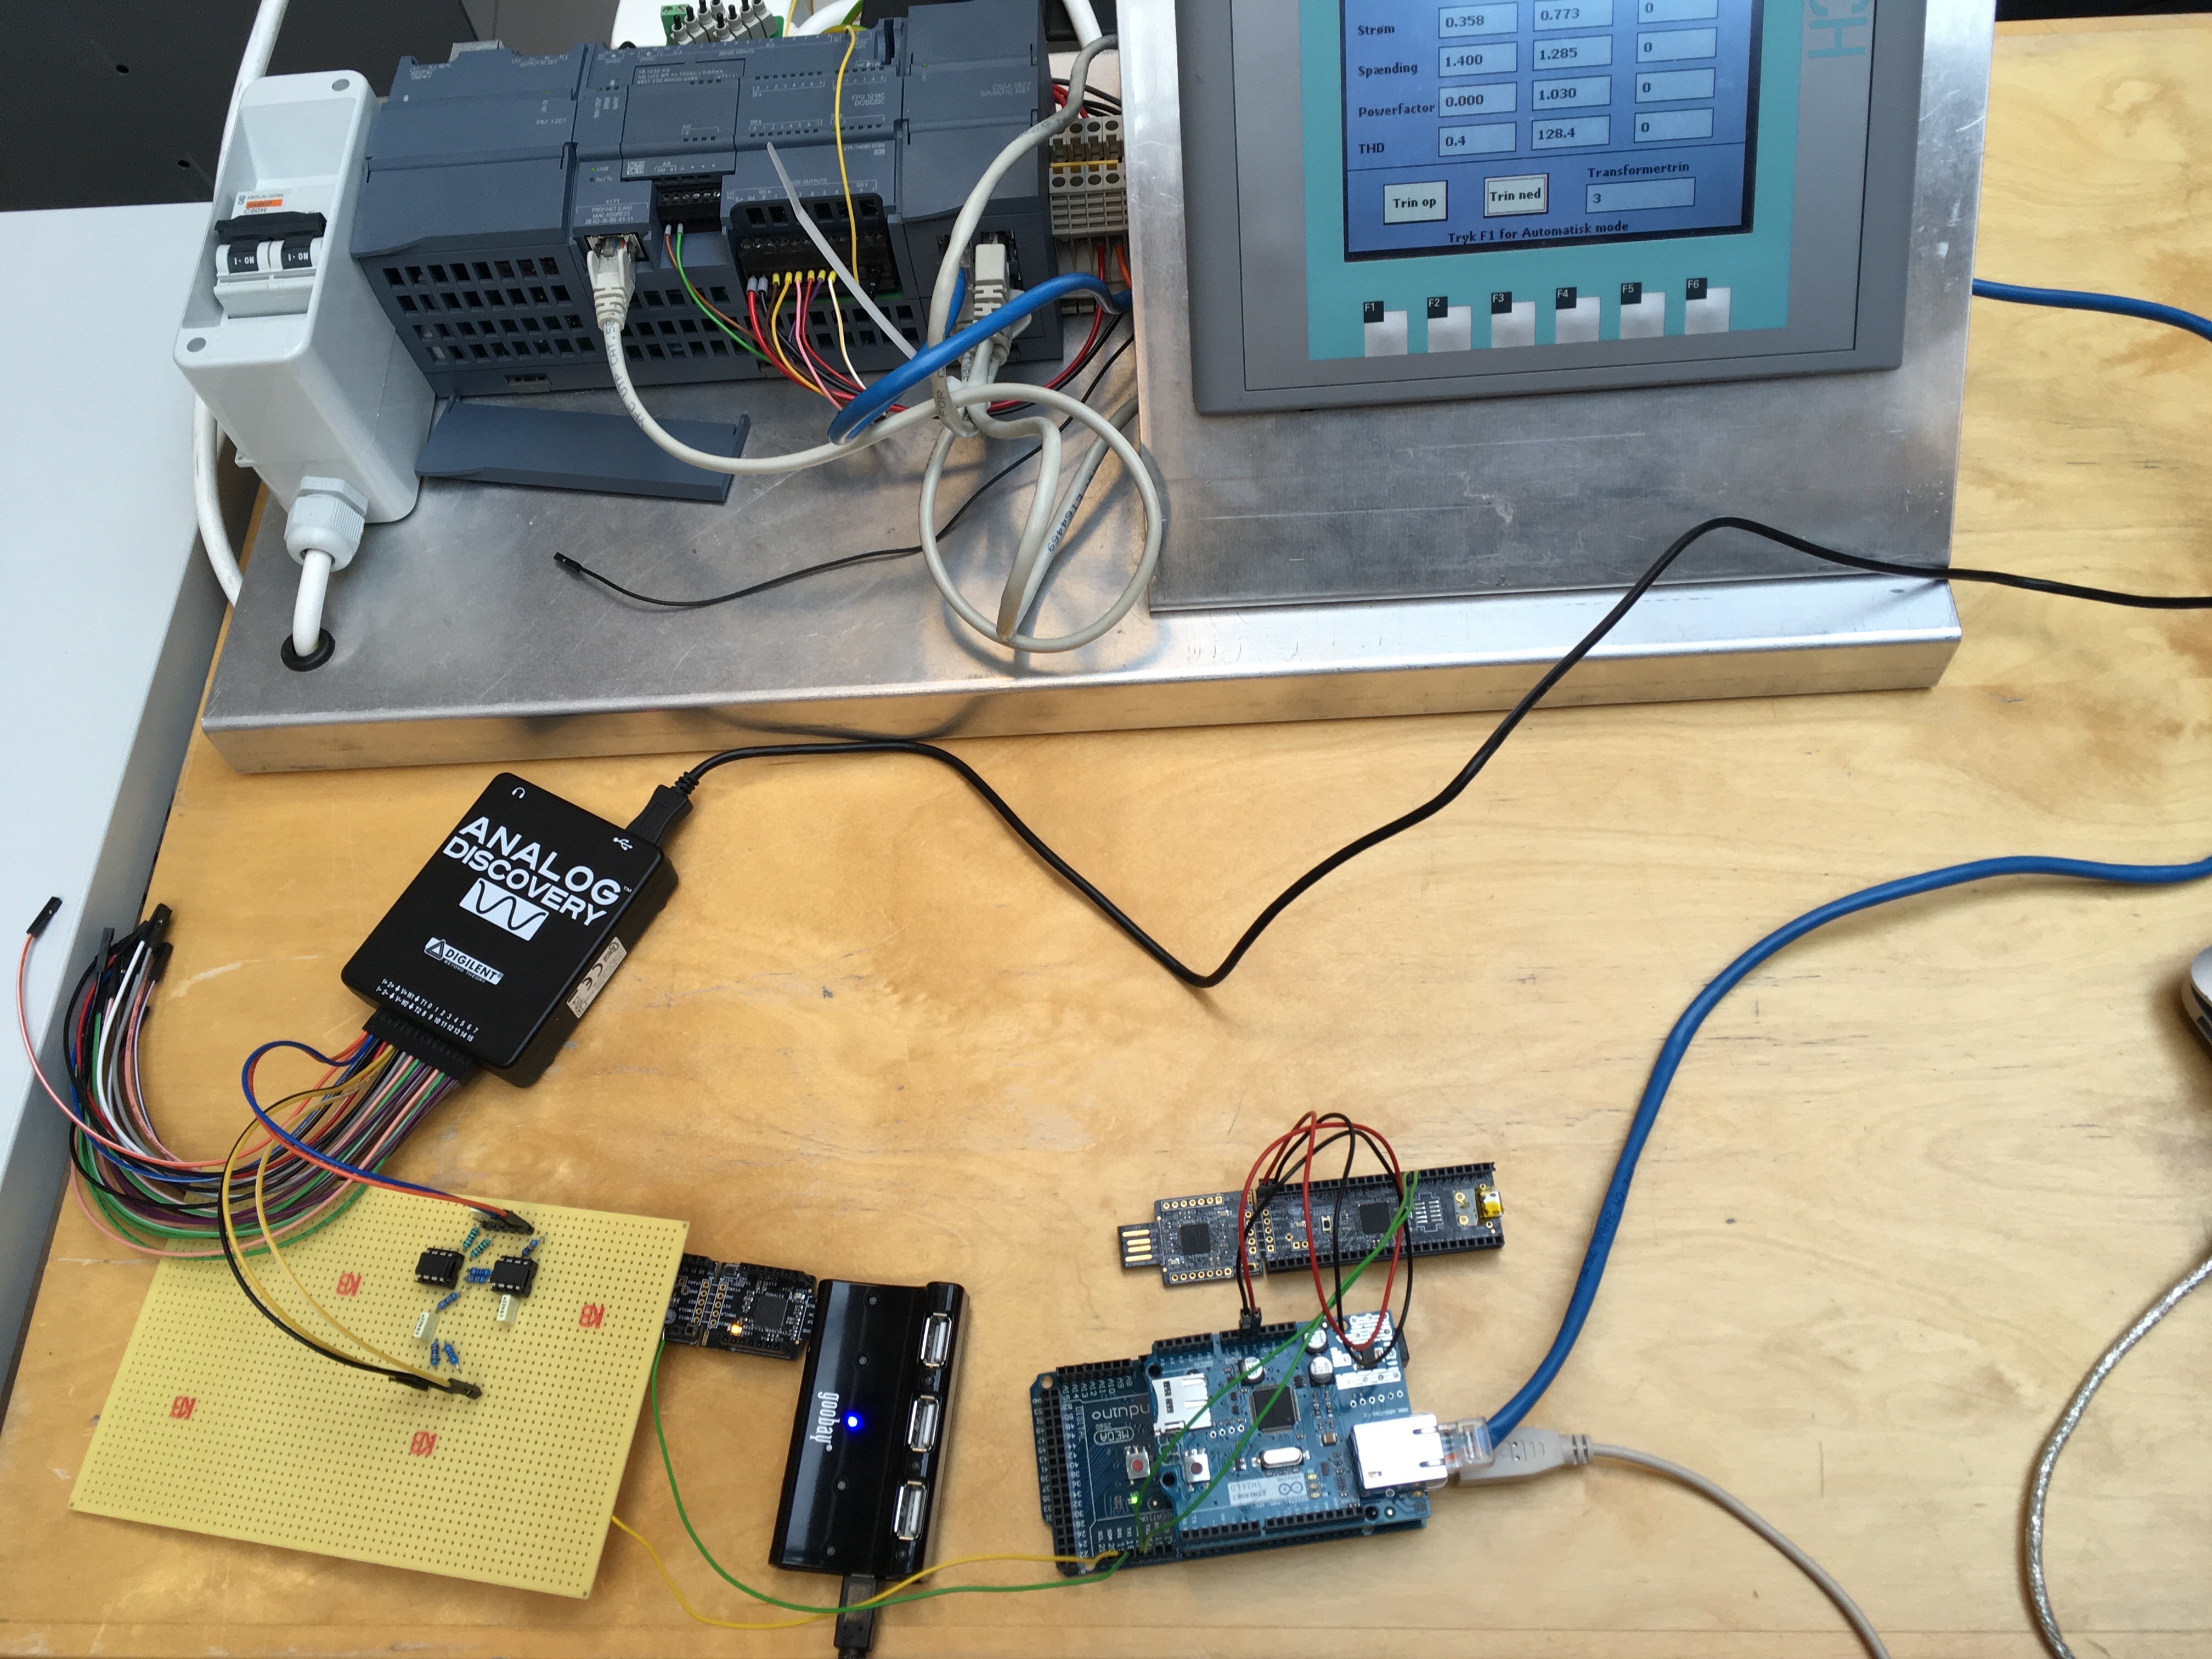
\includegraphics[width=0.7\textwidth]{Test/Opstilling1}
	\caption{Testopstilling af integrationstest mellem Måleenhed og Styringsenhed}
	\label{fig:opstilling1}
\end{figure}

Til testen skal der bruges:
\begin{itemize}
	\item 1 stk PSOC
	\item 1 stk Arduino med ethernet shield
	\item 1 stk PLC med hmi skærm
	\item Ledning fra PSOC's UART til Arduino
	\item Ethernet ledning fra ethrernet shield til PLC
\end{itemize}

\begin{center}
	\begin{tabular}{ | m{0.2\textwidth} | m{0.8\textwidth}|} 
		\hline
		\textbf{Test}					&Brugergrænsefladen modtager korrekte tal \\ \hline
		\textbf{Testbeskrivelse}		&Der testes at de værdiger, der kommer ind på Måleenheden er ens me værdigerne der vises på brugergrænsefladen. \\ \hline
		\textbf{Input}					&4VPP sinus på spænding indgang, 1VPP sinus på strøm indgang, 3,3ms forskydning \\ \hline
		\textbf{Forventet output}		&1,414V spænding, 0,354A strøm, 0,509 PF se figur \ref{fig:PFtest1}, 0 THD \\ \hline
		\textbf{Resultat}				&1,404V spænding, 0,359A strøm, 0,491, 0,2 THD,  se figur \ref*{fig:visningtest1} for resultat af skærm  \\ \hline
	\end{tabular}
\end{center}

\begin{figure}[H] % (alternativt [H])
	\centering
	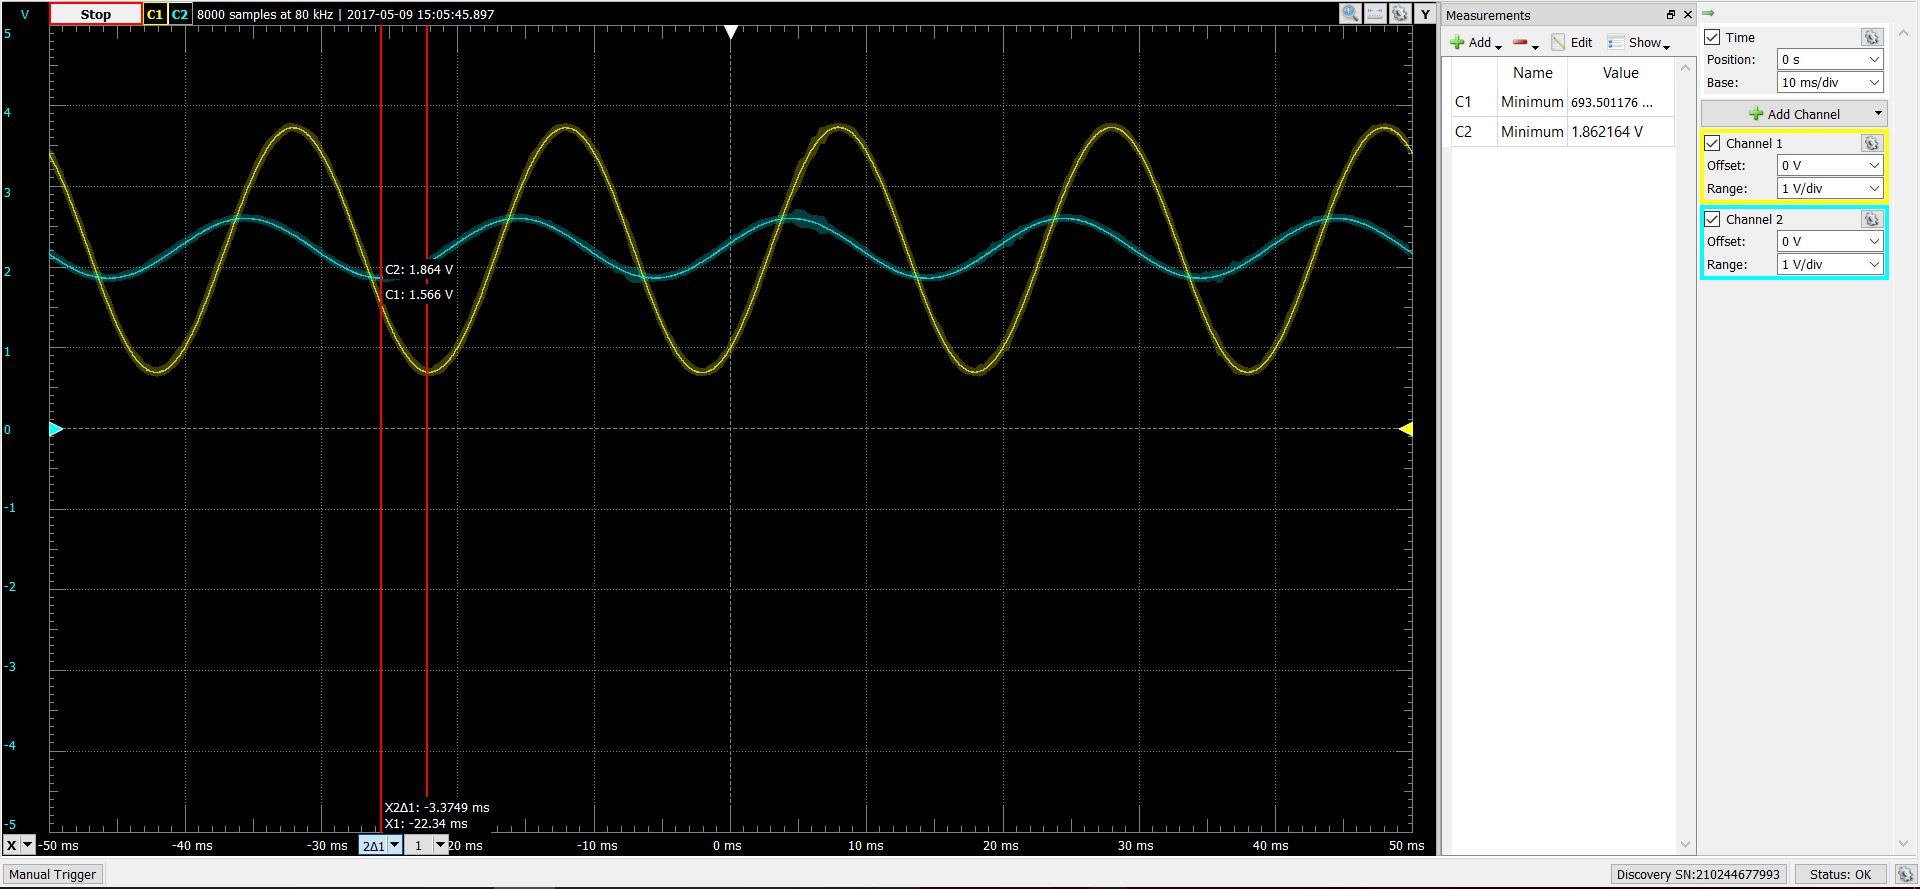
\includegraphics[width=0.7\textwidth]{Test/PFTest1}
	\caption{Visning af 3,3ms forsinkelse mellem strøm og spænding}
	\label{fig:PFtest1}
\end{figure}

\begin{figure}[H] % (alternativt [H])
	\centering
	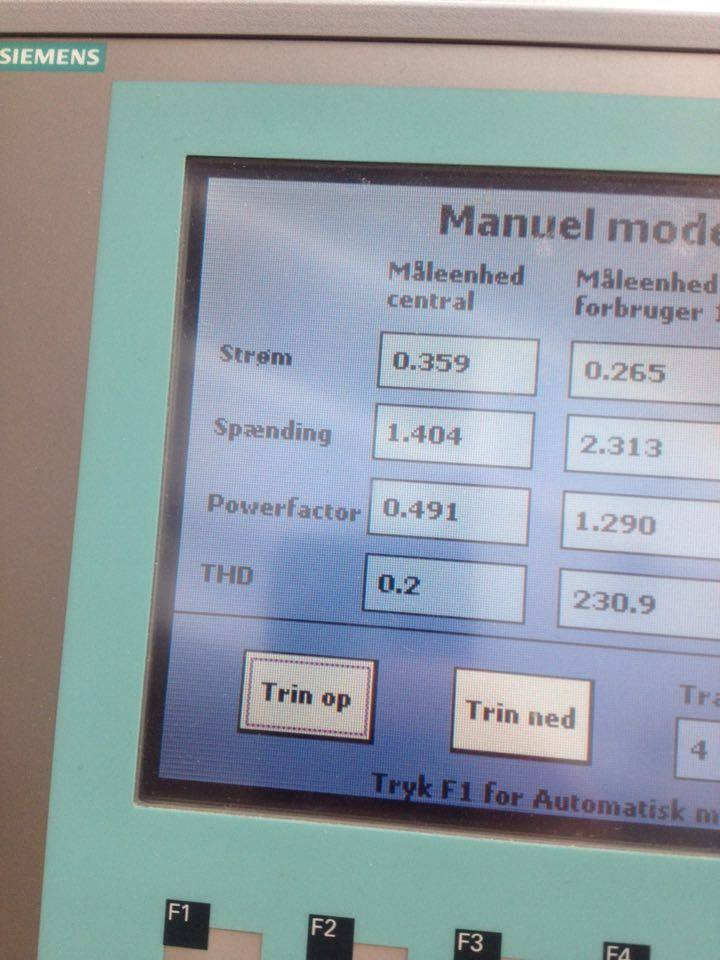
\includegraphics[width=0.5\textwidth]{Test/Visningstest1}
	\caption{Resultatet af visning på brugergrænseflade}
	\label{fig:visningtest1}
\end{figure}


\begin{center}
	\begin{tabular}{ | m{0.2\textwidth} | m{0.8\textwidth}|} 
		\hline
		\textbf{Test}					&Forsinkelse på brugergrænsefladen \\ \hline
		\textbf{Testbeskrivelse}		&Tiden der går fra mellem ændringer på skærmen \\ \hline
		\textbf{Input}					&4VPP \\ \hline
		\textbf{Forventet output}		&At der maks. går 2,5 sekund, pga intern delay i PLC og kommunikation \\ \hline
		\textbf{Resultat}				&2,01 2,00 1,99 2,00 1,95   \\ \hline
	\end{tabular}
\end{center}


\begin{center}
	\begin{tabular}{ | m{0.2\textwidth} | m{0.8\textwidth}|} 
		\hline
		\textbf{Test}					&Kommunikations pålidelighed \\ \hline
		\textbf{Testbeskrivelse}		&Der observeres på brugergrænsefladen i 1 min og tælles uregelmæssigheder \\ \hline
		\textbf{Input}					&4VPP sinus på spænding indgang, 1VPP sinus på strøm indgang\\ \hline
		\textbf{Forventet output}		&5\% fejl ud af 120 inputs \\ \hline
		\textbf{Resultat}				&5 fejl dvs. 4.17\%  \\ \hline
	\end{tabular}
\end{center}
